\section{Combinazione agli SLE frequente}
La $[2.5.3]$ delle \emph{NTC 2018} descrive la combinazione frequente per gli stati limite di esercizio reversibili.

\[
	G_1 + G_2 + \psi_{11}\cdot Q_{1k} + \psi_{22}\cdot Q_{2k} + \psi_{23}\cdot Q_{3k} + \dots
\]

Anche in questo caso vengono tralasciate le combinazioni che danno un contributo trascurabile.

\subsection{Calcolo delle azioni massime e minime}

\subsubsection*{Tratto $P13\div P16$}
\begin{equation*}
	\begin{cases}
		Q_{1,max} &= 8.00+11.52+3.75 + 11.55+7.98+9.20 + 0.2\cdot15.01 + 0.3\cdot(7.50+14.40) +0\\
		&= 61.572\,\dfrac{kN}{m}\\\\
		Q_{1,min} &= 8.00+11.52+3.75 + 11.55+7.98+9.20+0 + 0.5\cdot 7.50 + 0.3\cdot 14.40 +0\\
		&= 60.07\,\dfrac{kN}{m}
	\end{cases}
\end{equation*}

Il valore più alto corrisponde all'azione della neve, quello più basso corrisponde al carico di categoria del solaio intenro.

\subsubsection*{Tratto $P16\div P17$}
\begin{equation*}
	\begin{cases}
		Q_{2,max} &= 8.00+6.72+3.75 + 11.55+4.65+9.20 + 0.2\cdot10.30 + 0.3\cdot(7.50+8.40) + 0\\
		&= 50.70\,\dfrac{kN}{m}\\\\
		Q_{2,min} &= 8.00+6.72+3.75 + 11.55+4.65+9.20 +0+0.5\cdot 7.50 + 0.3\cdot 8.40+0\\
		&= 50.14\,\dfrac{kN}{m}
	\end{cases}
\end{equation*}

I valori corrispondono alle combinazioni del tratto precedente.

\subsubsection*{Tratto $P17$ - vano scala}
\begin{equation*}
	\begin{cases}
		Q_{3,max} &= 8.00+3.20+3.75 + 11.55+2.215+9.20 + 0+ 0.5\cdot7.50+ 0.3\cdot4.00 +0\\
		&= 42.865\,\dfrac{kN}{m}\\\\
		Q_{3,min} &= 8.00+3.20+3.75 + 11.55+2.215+9.20 + 0 + 0.3\cdot7.50 +0.5\cdot 4.00 + 0\\
		&= 42.165\,\dfrac{kN}{m}
	\end{cases}
\end{equation*}

Nel terzo tratto il massimo è generato dal sovraccarico di categoria interno, mentre il minimo dal sovraccarico di categoria della terrazza.

Di seguito si riportano gli  inviluppi delle sollecitazioni e le tabelle dei valori di riferimento.

\begin{figure}
	\centering
	\subfloat[\emph{Inviluppo dei momenti flettenti}]{
	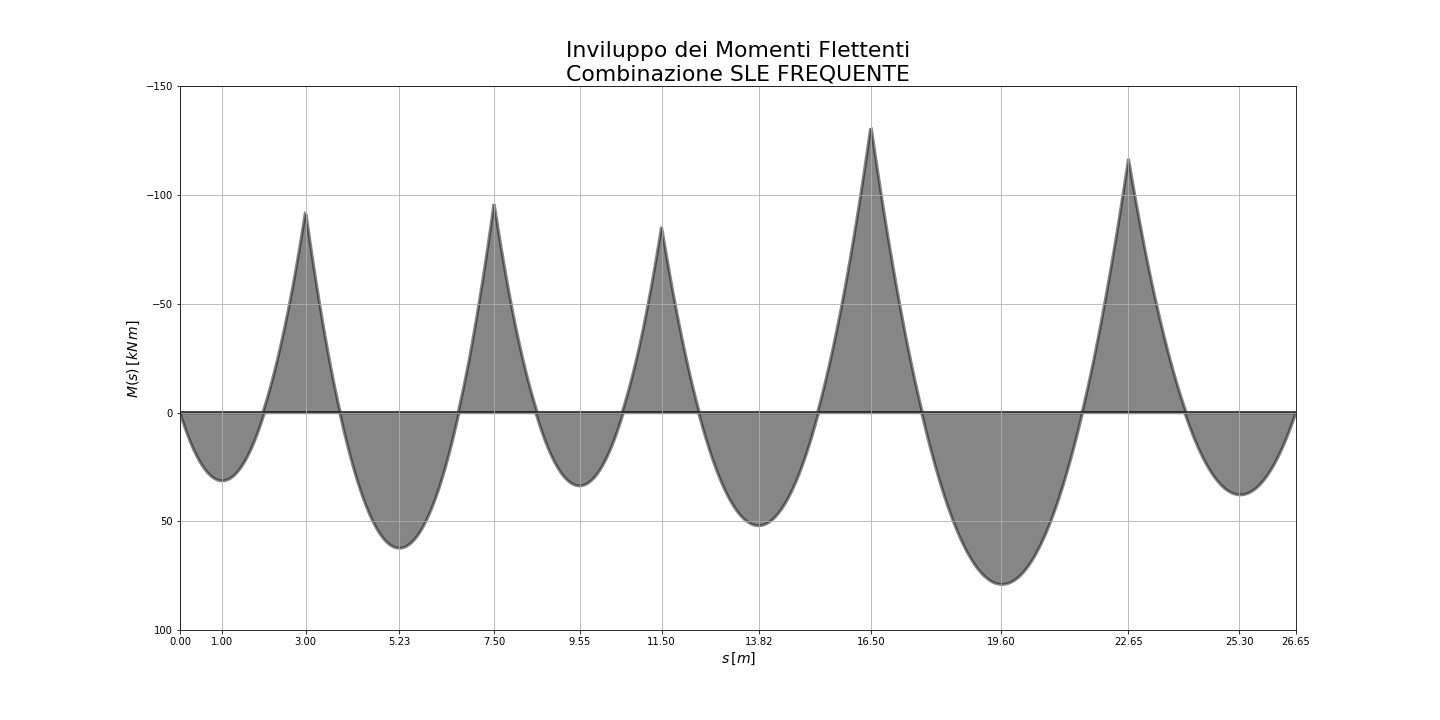
\includegraphics[width=.9\textwidth]{../../export/img/bendingMomentEnvelope_sleFreq}}\\
	\subfloat[\emph{Inviluppo dei tagli}]{
	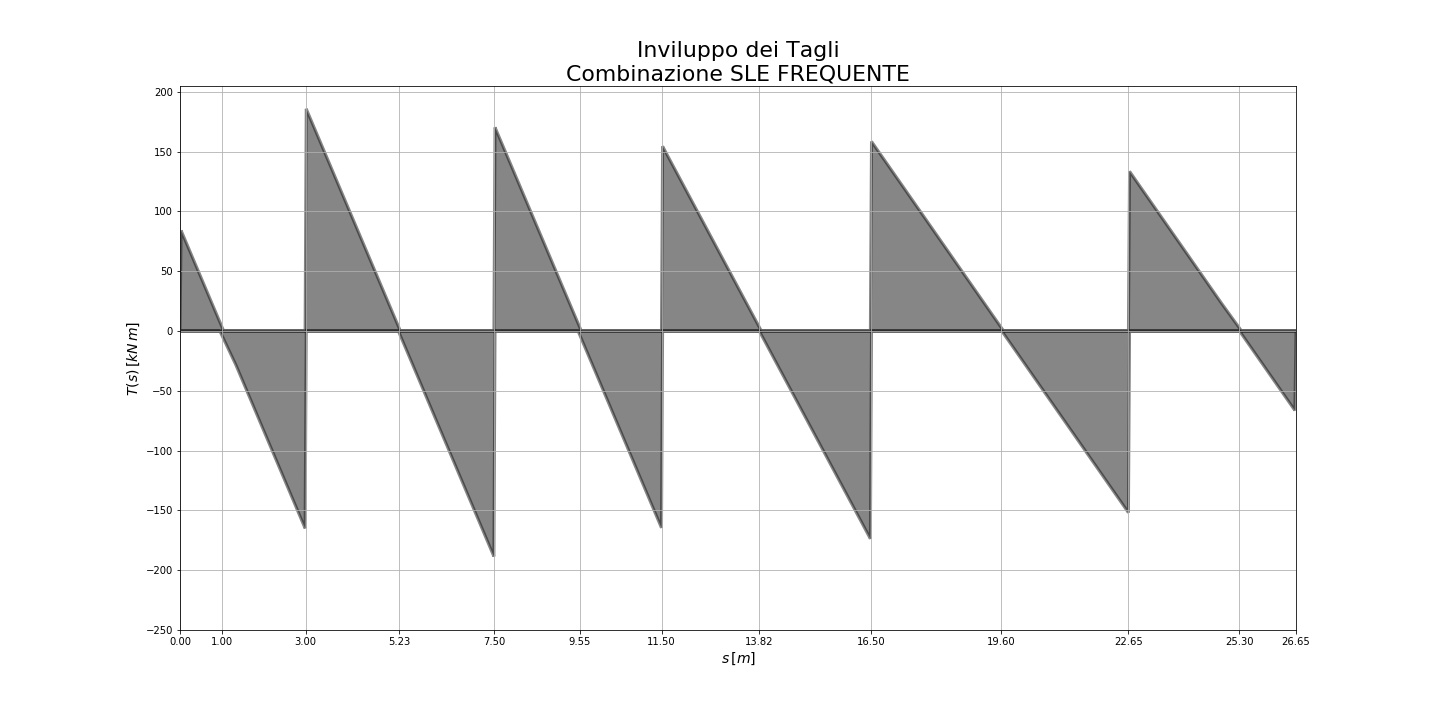
\includegraphics[width=.9\textwidth]{../../export/img/shearEnvelope_sleFreq}}
	\caption{Inviluppo delle sollecitazioni per la combinazione SLE frequente}
	\label{fig:sleFreqEnvelope}
\end{figure}

\begin{table}
  	\centering
  	\caption{Valori massimi e minimi dell'inviluppo dei momenti}
  	\label{tab:max_min_bendingMomentEnvelope_sleFreq}
  	\begin{tabular}{lcccr}
		\toprule
		& $M_{Ed}^+\,[kN\,m]$ & $s_{max}\,[m]$ & $M_{Ed}^-\,[kN\,m]$ & $s_{min}\,[m]$ \\
		Sezione &             &          &             &          \\
\midrule
C1      &     31.3916 &        1 &         NaN &      NaN \\
N2      &         NaN &      NaN &    -91.3156 &        3 \\
C2      &     62.3719 &     5.23 &           0 &      NaN \\
N3      &         NaN &      NaN &    -95.9325 &      7.5 \\
C3      &     33.7056 &     9.55 &           0 &      NaN \\
N4      &         NaN &      NaN &    -85.3944 &     11.5 \\
C4      &     52.0246 &    13.82 &           0 &      NaN \\
N5      &         NaN &      NaN &    -130.362 &     16.5 \\
C5      &     79.0371 &     19.6 &           0 &      NaN \\
N6      &         NaN &      NaN &    -116.735 &    22.65 \\
C6      &     37.8499 &       25 &         NaN &      NaN \\
\bottomrule
	\end{tabular}
  \end{table}
  
\begin{table}
  	\centering
  	\caption{Valori massimi e minimi dell'inviluppo dei tagli}
  	\label{tab:shearEnvelope_sleFreq}
  	\begin{tabular}{lcccr}
		\toprule
		& $T_{Ed}^+\,[kN]$ & $s_{max}\,[m]$ & $T_{Ed}^-\,[kN]$ & $s_{min}\,[m]$ \\
		Sezione &             &          &             &          \\
		\midrule
N1      &    84.006 &        0 &         0 &        0 \\
N2      &   185.787 &        3 &  -165.029 &        3 \\
N3      &   170.316 &      7.5 &  -188.546 &      7.5 \\
N4      &   154.466 &     11.5 &  -164.588 &     11.5 \\
N5      &   158.492 &     16.5 &  -173.737 &     16.5 \\
N6      &    133.49 &    22.65 &   -151.89 &    22.65 \\
N7      &         0 &    26.65 &  -66.4499 &    26.65 \\
		\bottomrule
	\end{tabular}
  \end{table}

\cleardoublepage
